\documentclass[a4paper,12pt]{article}
\usepackage[english,ukrainian,russian]{babel}
\linespread{1}
\usepackage{ucs}
\usepackage[utf8]{inputenc}
\usepackage[T2A]{fontenc}
\usepackage[paper=portrait,pagesize]{typearea}
\usepackage{amsmath}
\usepackage{bigints}
\usepackage{amsfonts}
\usepackage{graphicx}
\usepackage{amssymb}
\usepackage{cancel}
\usepackage{gensymb}
\usepackage{multirow}
\usepackage{rotate} 
\usepackage{pdflscape}
\usepackage{bigstrut}
\usepackage[pageanchor]{hyperref}
\usepackage{chngpage}
\newcommand{\dx}{\textbf{d}x}
\newcommand{\dt}{\textbf{d}t}
\newcommand{\du}{\textbf{d}u}
\newcommand{\dv}{\textbf{d}v}
\newcommand{\dy}{\textbf{d}y}
\newcommand{\ds}{\textbf{d}s}
\newcommand{\dz}{\textbf{d}z}
\newcommand{\arch}{\textrm{arcch}}
\newcommand{\arsh}{\textrm{arcsh}}
\newcommand{\dint}{\displaystyle\int}
\newcommand\tab[1][1cm]{\hspace*{#1}}
\newcommand{\dsum}{\displaystyle\sum}
\newcommand{\RomanNumeralCaps}[1]{\MakeUppercase{\romannumeral #1}}
\usepackage[left=20mm, top=20mm, right=15mm, bottom=15mm, nohead, nofoot]{geometry}
\usepackage{verbatim}

\usepackage{listings}
\usepackage{xcolor}

\definecolor{codegreen}{rgb}{0,0.6,0}
\definecolor{codegray}{rgb}{0.5,0.5,0.5}
\definecolor{codepurple}{rgb}{0.58,0,0.82}
\definecolor{backcolour}{rgb}{0.95,0.95,0.92}

\lstdefinestyle{mystyle}{
	backgroundcolor=\color{backcolour},   
	commentstyle=\color{codegreen},
	keywordstyle=\color{blue},
	numberstyle=\tiny\color{codegray},
	stringstyle=\color{red},
	basicstyle=\ttfamily\footnotesize,
	breakatwhitespace=false,         
	breaklines=true,                 
	captionpos=b,                    
	keepspaces=true,                 
	numbers=none,                    
	numbersep=5pt,                  
	showspaces=false,                
	showstringspaces=false,
	showtabs=false,                  
	tabsize=4,
	frame=shadowbox
}

\lstset{style=mystyle}


\begin{document}
\begin{center}
    \hfill \break
    \large{\textbf{НАЦIОНАЛЬНИЙ ТЕХНIЧНИЙ УНIВЕРСИТЕТ УКРАЇНИ\\
            «КИЇВСЬКИЙ ПОЛIТЕХНIЧНИЙ IНСТИТУТ»\\
            НАВЧАЛЬНО-НАУКОВИЙ ФІЗИКО-ТЕХНІЧНИЙ ІНСТИТУТ}}\\
    \hfill \break \hfill \break \hfill\break \hfill \break \hfill \break \hfill \break \hfill \break
    \hfill \break \hfill \break \hfill \break \hfill \break
    \large{Лабораторна робота № 1}
    \begin{center}
        \normalsize{\textbf{з дисципліни «Алгоритми та структури даних» \\
        На тему: «Рекурсивні алгоритми» \\}}
    \end{center}
\end{center}
\hfill \break \hfill \break \hfill \break \hfill \break \hfill \break \hfill \break \hfill \break
\hfill \break \hfill \break \hfill \break \hfill \break \hfill \break \hfill \break 
\begin{flushright}
    \large{ \hspace{35pt} Виконав:\\
        студент групи ФI-12\\
        Завалій Олександр} 
\end{flushright}
\hfill \break \hfill \break \hfill \break \hfill \break \hfill \break \hfill \break \hfill \break
\hfill \break
\begin{center} \textbf{Київ-2023} \end{center}
\thispagestyle{empty}

\newpage
    \begin{center}
        \section*{\bfseries{Реалізація завдання}}
    \end{center}
    \begin{center}
        \Large{Task \RomanNumeralCaps{2}}
    \end{center}
    \textbf{Знайти НСД двох цілих чисел за алгоритмом Евкліда.}
    \begin{figure}[h!]
        \begin{minipage}[h]{1\linewidth}
            \centering
            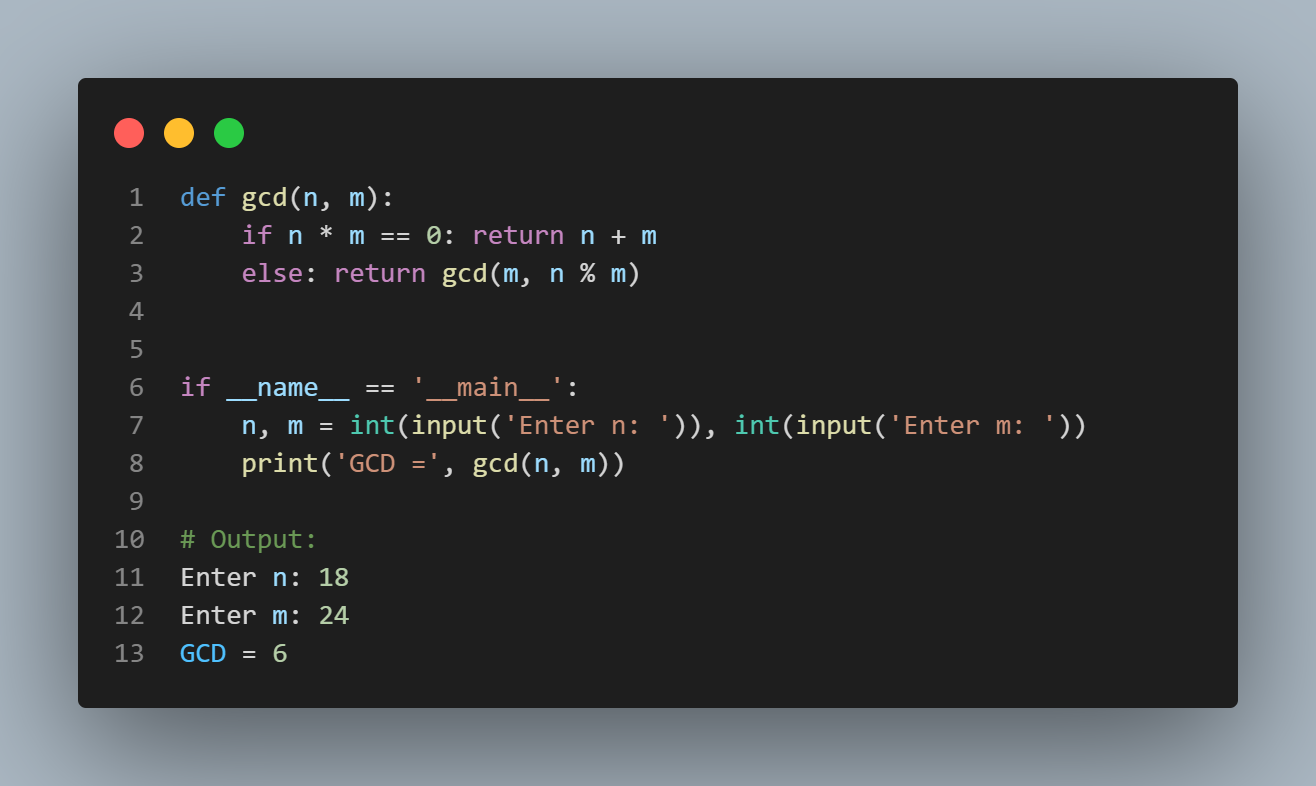
\includegraphics[width=0.9\linewidth]{Prt sc/Figure_1.png}  
        \end{minipage}
    \end{figure}
\end{document}